\documentclass[20pt,,margin=1in,innermargin=-4.5in,blockverticalspace=-0.25in]{tikzposter}
\geometry{paperwidth=42in,paperheight=32.5in}

\usepackage[utf8]{inputenc}
\usepackage{amsmath}
\usepackage{amsfonts}
\usepackage{amsthm}
\usepackage{amssymb}
\usepackage{mathrsfs}
\usepackage{graphicx}
\usepackage{adjustbox}
\usepackage{enumitem}
\usepackage[backend=biber,style=numeric]{biblatex}
\usepackage{SUtheme}

\usepackage{mwe} % for placeholder images
\usepackage{import}
\usepackage{caption}

\addbibresource{bib.bib}

% set theme parameters
\tikzposterlatexaffectionproofoff
\usetheme{SUTheme}
\usecolorstyle{SUStyle}
\usetitlestyle{Filled}

\usepackage[scaled]{helvet}
\renewcommand\familydefault{\sfdefault} 
\usepackage[T1]{fontenc}

\usepackage{wrapfig}
\usepackage{svg}
\usepackage{import}

\title{Volumetric Ray Tracing}
\author{Matthias Eberhardt}
\institute{Ostbayerische Technische Hochschuler Regensburg}
\titlegraphic{\includegraphics[width=0.06\textwidth]{oth.png}}

% begin document
\begin{document}
\maketitle
\centering
\begin{columns}
    \column{0.5}
    \block{Motivation}{
    In Computer Graphics, objects usually are represented as a set of geometric primitives (e.g. triangles), displaying the surface of the object. However, if a volumtric object (e.g a cloud), is to be rendered, the traditional rendering technique requires an intermediate surface representation that can introduce unwanted artifacts. Volumetric ray tracing provides a mechanism to directly render such 3D data without the need for a surface representation.
    
    }
    
    
    \block{Participating Media and the Beer-Lambert Law}{
      \begin{wrapfigure}{l}{0.25\columnwidth}\label{fig:interactions}
\def\svgwidth{0.25\columnwidth}
  \import{figures/}{fig_interactions.pdf_tex}
  \caption{Light interactions in participating media.}
  \end{wrapfigure}
   Surface ray tracing calcualtes the light point $x$ receives from the nearest surface point $y$ in direction $-\omega$. This quantity is called $L_e(y,\omega)$. Surface ray tracing then makes the assumption that the light experiences no changes during its travel:
   \begin{align*}
   L(x,\omega) = L_e(y, \omega)
   \end{align*}
   This assumption holds only true if the light travels through a vacuum, if it travels through a medium that interacts with it (called a participating medium), the intensity changes. The possible interactions (see figure \ref{fig:interactions}) include absorption (e.g. in smoke), in and out-scattering (e.g. in clouds), and emission from within the medium that add light to the ray (e.g. in fire). The goal of volumetric ray tracing is to correctly model those interactions.
  

  
        %\begin{tikzfigure}[Interactions in participating media]\label{fig:interactions}
         %   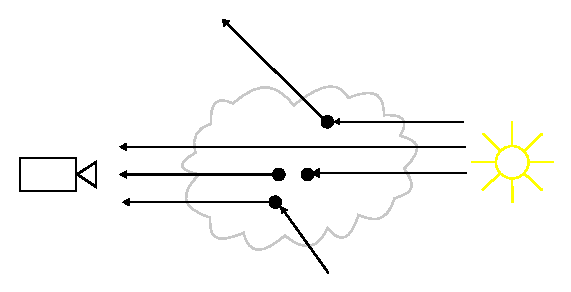
\includegraphics[width=0.3\linewidth]{fig_interactions.eps}
        %\end{tikzfigure}

   
         The interactions enumerated above occur due to tiny particles suspended within the medium, which are stochastically modeled by the absorption coefficient $\mu_a(x)$ and scattering coefficient $\mu_s(x)$,  providing a measure for the light loss lost due to out-scattering and absorption respectively. Combining $\mu_a$ and $\mu_s$ to the extinction coefficient $\mu_t$ gives a measure for the total amount of light lost. Using the Beer-Lambert law, the attenuation or transmittance between $x$ and $y$ is calculated as 
         \begin{align*}
         \tau(x,y) = e^{-\int_{x}^{y}\mu_t(s)ds}
         \end{align*}
         This describes the percentage of light that ``survives'' the travel from $x$ to $y$.
    }
    \block{Mathematical Model}{
    
    
    \begin{wrapfigure}{l}{0.25\columnwidth}\label{fig:light_changes}

\def\svgwidth{0.25\columnwidth}
  \import{figures/}{fig_light_changes.pdf_tex}
  \caption{TEst.}
  \end{wrapfigure}
  
  
     Thus, $L_e$ gets attenuated by $\tau(x,y)$. Furthermore, for every point $u$ between $x$ and $y$, the ray intensity changes due to emission and in-scattering. Emission is calculated as $\mu_a(u)\varepsilon(u, \omega)$, in-scattering as $\mu_s\int_{\Omega}f_p(u,\omega,-\omega')L(u,\omega')d\omega'$, where $\varepsilon(u,\omega)$ is the light emitted by a particle at $u$ in direction$\omega$, and $f_p$ is the phase function, which describes the probabilty that light arriving from $-\omega'$ is scattered towards $\omega$. 
     \newline
     Therefore, the light send from $u$ to $x$ is 
     \begin{align*}
     L_e^s(u,\omega) = \mu_s\int_{\Omega}f_p(u,\omega,-\omega')L(u,\omega')d\omega' + \mu_a(u)\varepsilon(u, \omega)
     \end{align*}
     The total added light intensity to the ray between $x$ and $y$ is computed by the line integral of $L_e^s$. Adding this to the attenuated light from $y$  results in the rendering equation
     \begin{align*}
     L(x, \omega) = \int_{x}^{y}\tau(x,u)L_e^s(u,\omega)du + L_e(y,\omega)
     \end{align*} 
    }

    \column{0.5}
    \block{Discrete Ray Marching}{
    
    }
    
    \block{Monte Carlo Ray Tracing}

    
    \block{References}{
        \vspace{-1em}
        \begin{footnotesize}
        \printbibliography[heading=none]
        \end{footnotesize}
    }
\end{columns}
\end{document}
